\documentclass{article}

\usepackage{amsmath}
\usepackage{float}
\usepackage{csvsimple}

\usepackage{graphicx}
\graphicspath{ {../results/} }

\usepackage[style=numeric, backend=bibtex8]{biblatex}
\addbibresource{citations.bib}

\begin{document}

  \title{Linear Time Generation of Simulated Wireless Sensor Networks with Random Geometric Graphs}
  \author{Luke Wood}
  \maketitle

  \section{Executive Summary}
	Wireless Sensor Networks (WSNs) are a group of ad hoc wireless devices that communicate amongst themselves.
  WSNs have tons of applications coming in the near future ranging from traffic sensing networks to weather reading sensors on the surface of Mars\cite{mahjoub2010employing}.
	They are incredibly expensive to develop and test which makes them a great candidate for simulation as a preliminary way to gather data.
	Vlady Ravelomananana and Hichem Kenniche from the University of Paris first explored the concept of using random geometric graphs (RGGs) to attempt to model wireless sensor networks \cite{kenniche2010random}.
  At the moment random geographic graphs are the state of the art method for simulating WSNs.
	In this project I will use RGGs as a way to gather valuable information about how wireless sensor networks will possibly function and communicate.

  \subsection{Introduction and Summary}
	Through a series of three reports	I will be analyzing RGGs in the following ways as an attempt to gain some insight into the behavior of wireless sensor networks:
	\begin{enumerate}
		\item Generating RGGs on the geometries of a unit square, unit disc, and unit sphere
		\item Color the generated graph in linear time using smallest vertex last ordering\cite{matula1983smallest}
		\item Find the terminal clique in the generated RGGs
		\item Find a selection of bipartite subgraphs producted by an algorithm for coloring
	\end{enumerate}
	This report is the first of the series and will describe an implementation for a linear time algorithm to generate graphs consisting of N vertices with an average degree of A on the geometric topologies of: unit square, unit disc, unit sphere.
	Some tables are included to display some metrics for generated  RGGs of various size to display the performance of the generation algorithm.
	The square topology generation algorithm runs in approximately 15 seconds for graph size 100000 which is fast given the large input size.
  Reference table \ref{square_benchmarks} for in depth information on this algorithm.
  \begin{table}
    \centering
    \label{square_benchmarks}
    \csvautotabular{../results/square/benchmarks/data.csv}
		\caption{Data on Graphs Generated with the Square Topology}
	\end{table}

	The disc topology also runs in linear time but the constant factor is much larger than that of the square topology.
	This is due to some overhead that I incurred when generating the points themselves.
	Despite the algorithm being slower than the square version, it still terminated in 48 seconds for 100000 nodes.
  At the moment this is the worst generation algorithm and could be improved by using mathematical formulas instead of repeated guessing to generate points.
  Reference table \ref{disc_benchmarks} for in depth information on this algorithm.

  \begin{table}
    \centering
    \label{disc_benchmarks}
    \csvautotabular{../results/disc/benchmarks/data.csv}
		\caption{Data on Graphs Generated with the Disc Topology}
	\end{table}

  Sphere generation was also a linear time algorithm.
  Unlike the disc topology I generated the points using a mathematical formula instead of brute force finding points.
  Thie yielded a runtime of under 35 seconds for generating 32000 points.
  Reference table \ref{sphere_benchmarks} for in depth information on this algorithm.

  \begin{table}
    \centering
    \label{sphere_benchmarks}
    \csvautotabular{../results/sphere/benchmarks/data.csv}
		\caption{Data on Graphs Generated with the Sphere Topology}
	\end{table}

	One interesting thing to notice in the tables is that as the number of nodes grows the real average degree converges on the expected average degree.
	The lower the number of nodes the further from the expected average degree the real number is.
	This happens due to there not being enough nodes in the graph for the real radius to reach the expected value.
  The random error in the point generation is more apparent when there are fewer nodes in the graph.

	Going forwards I will continue to implement linear time algorithms to solve the problems at hand.
	I will possible move from python to the Elixir programming environment to utilize the high level of parralelism and the huge speed gain from type inference.

  Currently, my implementation has support for:
  \begin{enumerate}
		\item Generating a RGG with a unit square topology
		\item Generating a RGG with a unit disc topology
    \item Generating a RGG with a unit sphere topology
		\item Converting RGGs to an Adjacency List
		\item Serializing Adjacency Lists to files
  \end{enumerate}

  \subsection{Programming Environment Description}
		The implementation of the algorithm used to gather the data supporting this report was gathered on a 15 inch Macbook pro 2017 with a 2.9 GHz Intel Core i7 processor and 16 GB of RAM.
		The computer is running macOS High Sierra.
		The graph generation is written in python 3 as generating and connection a graph is not super computationally expensive with even decently large inputs such as 100000 (assuming $O(n) algorithms$).
		The later algorithms may be implemented in a different language such as Elixir to get high levels of concurrency and higher efficiency due to type inference (as opposed to python's dynamic typing).
  \section{Reduction to Practice}
    This section will describe the transition from theory to implementation.
    This section will also give a detailed analysis of the algorithms used in this project as well as their asymptotic runtimes.
	\subsection{Data Structure Design}
		The generation portion of this project uses several different data structures.
		The first one is a python object of custom type node.
		This serves as a tuple of values consisting of a list of dimensions, a list of nodes, and a node number.
		The first two are used during graph generation and the latter during conversion to an adjacency list.
		This data structure could be used interchangeably with a statically indexed tuple instead of an object to avoid any overhead associated with objects in python, however the readability gained from using a custom node class heavily outweighs the marginal performance benefit gained from using a statically indexed tuple.
		Both of these data structures provide $O(1)$ read and write operations.
		If the goal were to generate gigantic graphs then an argument could be made to switch over the statically indexed tuples to reduce the access time for attributes by a bit as tuples use static memory address offsets.

		The second mentioned data structure is the adjacency list.
		Adjacency lists are an efficient graph representation that we will use in the subsequent reports.
		Adjacency lists require only $O(v*e)$ storage as opposed to the $O(v^2)$ required for adjacency matrixes.
		This is handy in situations where the expected average number of edges is significantly lower than the number of nodes in the graph.
		Despite the huge potential savings on storage, the only sacrifice adjacency lists make is in the lookup operation to determine if there is an edge between two nodes.
		This takes $O(e)$ in an adjacency list as opposed to $O(1)$ in an adjacency matrix.

	\subsection{Algorithm Description}
		This section gives a detailed analysis of the algorithms used in the graph generation implementation.
    Table \ref{asymptotic_runtime_table} contains information on the asymptotic runtimes of the algorithms in terms of $O$ and $\Omega$.
		\begin{table}
      \centering
      \label{asymptotic_runtime_table}
			\begin{tabular}{ |c|c|c| }
				\hline
				Algorithm & $\Omega$ & $O$ \\
				\hline
				Square Point Generation & $\Omega(n)$ & $O(n)$ \\
				\hline
				Disc Point Generation & $\Omega(n)$ & $O(n)$ \\
				\hline
        Sphere Point Generation & $\Omega(n)$ & $O(n)$ \\
        \hline
				Node Connection & $\Omega(n)$ & $O(n)$ \\
				\hline
			\end{tabular}
      \caption{big $O$ and big $\Omega$ of all of the algorithms described}
		\end{table}

  \paragraph{Square Point Generation}
		The algorithm to generate the points in the unit square topology is simple.
		The steps are as follows:
    \begin{enumerate}
      \item x=random(0, 1), y=random(0, 1)
      \item add (x,y) to a list of points
      \item repeat steps 1 and 2 until N points are created
    \end{enumerate}
    That is all that is necesary to get a random point in the unit square.
    This algorithm is $\Theta(n)$.

  \paragraph{Disc Point Generation}
		Generating the points on the disc topology is slightly more challenging than generating the points for the square topology.
    The algorithm for generating points used in the implementation descriped in this point is as follows:
    \begin{enumerate}
      \item x=random(0, 1), y=random(0,1)
      \item if the distance from (x,y) to (.5, .5) is < .5, add (x,y) to a list of points
      \item repeat steps 1 and 2 until N points are created
    \end{enumerate}
    The issue with this algorithm is the nondeterminism involved in creating each point.
    When generating large numbers of points lots of work is wasted on generating the unused random points.
    In future iterations of this project a mathematical approach may be used to generated these points.
    Despite the non-determinism, this algorithm is still amortized $\Theta(n)$.

    A possible approach to fixing this implementation would be to pick a radius between 0 and 1, and then rotate by a random number of radians between 0 and 2$\pi$.
    This was not implemented as I was unsure if this would produce a uniform distribution.

  \paragraph{Sphere Point Generation}
    Generating points on the surface of the unit sphere can be solved using math.
    The steps for the following algorithm are as follows:

    \begin{enumerate}
      \item u = (random() * 2) - 1, theta = random() * 2 * pi
      \item x = sqrt(1 - u**2) * cos(theta), y = sqrt(1 - u**2) * sin(theta), z = u
      \item append (x, y, z) to a list of points.
      \item repeat steps 1-3 N times
    \end{enumerate}

    In the implementation associated with this report the values x, y, and z are transformed to form a sphere around (.5, .5, .5) as opposed to (0, 0, 0) as it makes the connection algorithm simpler.
    This algorithm is $\Theta(n)$.

	\subsection{Node Connection}
		In order to ensure that average degree of the nodes is close to the desired average degree, a radius of a specific length can be defined surrounding each node.
    The nodes within that radius of each other are then connected in the graph.
		The formulas to find the radius for each topology is derived from the equations found in the paper Bipartite Grid Partitioning of a Random Geometric Graph\cite{chen2017bipartite}.
		The formula used to find this radius varies for each graph tolopogy and can be found in the table \ref{radius_equations}.

    \begin{table}
      \centering
      \label{radius_equations}
  		\begin{tabular}{ |c|c|c| }
  				\hline
  				Topology & Equation Used to Derive Radius & Radius Equation \\
  				\hline
  				Unit Square & $d(G) \approx N\pi r^2 $ & $r = sqrt(\dfrac{d(G)}{N\pi})$ \\
  				\hline
  				Unit Disc & $r = sqrt(\dfrac{d(G)}{N\pi})$ & $r = sqrt(\dfrac{d(G)}{N})/2$ \\
  				\hline
  				Unit Sphere & $r = sqrt(\dfrac{d(G)}{N})/2$ & $r = sqrt(\dfrac{d(G)}{N})*2/3$ \\
  				\hline
  		\end{tabular}
    \end{table}

    The brute force algorithm for generating and connecting RGGs in this way is $O(n^2)$.
    This quickly became problematic as the algorithm took upwards of 200 seconds to run on input size of only 12,000.
    Figure \ref{brute_force_runtimes} shows this issue.
    \begin{figure}
      \centering
      \label{brute_force_runtimes}
      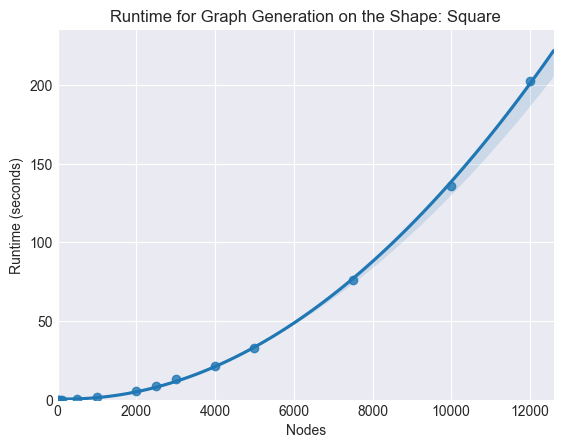
\includegraphics[width=1 \textwidth]{square/runtime/runtime_chart_naive}
      \caption{Runtimes of the $O(n^2)$ Algorithm}
    \end{figure}
    Instead, the implementation uses a bucket method to narrow down the required number of comparisons.
    The idea for this algorithm comes from the paprer Bipartite Grid Partitioning of a Random Geometric Graph\cite{chen2017bipartite}.
    The algorithm can be broken down into steps as follows:

    \begin{enumerate}
      \item create $(\sqrt{1/R} - 1 )^2$ buckets
      \item place buckets in a 2D grid arrangement
      \item for each node, place the node in bucket (x, y) such that x=$floor(x*num_buckets)$, y=$floor(y*num_buckets)$
      \item for each x,y such that x=0..buckets, y=0..buckets
      \item check to see if each node in bucket (x,y) is within radius R to all others in bucket (x,y) as well as (x+1,y-1), (x+1,y), (x,y+1), (x+1,y+1)
      \item if two nodes are under radius R from each other, place an edge between them.
    \end{enumerate}
    This algorithm is $O(n)$ given a small enough radius and a sufficient number of buckets.
    This means that with sufficiently many nodes and as long as the expected average degree remains low the algorithm will be linear.
    The runtimes for the implementation of this algorithm can be found in figure \ref{optimised_runtimes_for_connection}.
    \begin{figure}
      \centering
      \label{optimised_runtimes_for_connection}
  		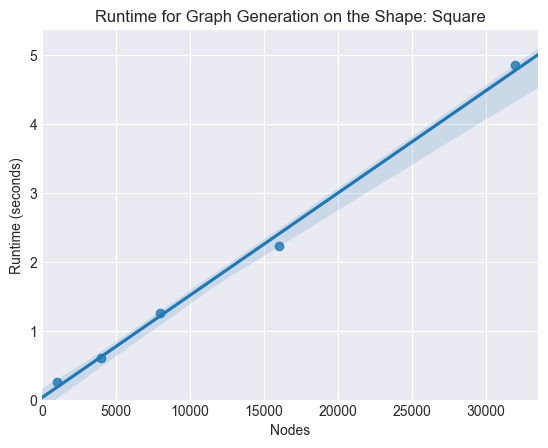
\includegraphics[width=1 \textwidth]{square/runtime/runtime_chart}
  		\caption{Runtimes of the $O(n)$ Algorithm}
	  \end{figure}

	\paragraph{Conversion From Node List to Adjacency Matrix}
    The algorithm to convert from a node list to an adjacency matrix is as follows:
    \begin{enumerate}
      \item map each node to it's edge list attribute
      \item map each edge list to the contained nodes' node numbers
    \end{enumerate}
		This quickly yields an $O(v*e)$ algorithm to change my node list to an adjacenecy matrix.
		If the performance of $O(v*e)$ is deemed unacceptable in the future, then we can simply append the node number to the list of edges as opposed to a pointer to the node object deeming the second map operation unneccesary yieling an $O(v)$ algorithm.
  \subsection{Algorithm Engineering}
    As mentioned above, the brute force algorithm to find adjacent nodes becomes slow at a fast rate.
    To fix this, the implementation presented uses linear time algorithms for all of it's operations.
	  Table \ref{runtime_comparison_table_brute} compares the runtimes of the linear implementation to that of the quadratic implementation.

	  \begin{table}
      \centering
      \label{runtime_comparison_table_brute}
  		\begin{tabular}{ |c|c|c| }
  			\hline
  			Nodes & $O(n^2)$ & $O(n)$ \\
  			\hline
  			  1000 & 0.258400 & 0.657174 \\
  			  \hline
  			  2000 & 0.382116 & 2.630040 \\
  			  \hline
  			  3000 & 0.473916 & 5.874501 \\
  			  \hline
  			  5000 & 0.831753 & 16.809004 \\
  			  \hline
  			  10000 & 1.560216 & 65.398991 \\
  			\hline
  		\end{tabular}
  		\caption{Runtimes of the $O(n)$ and $O(n^2)$ algorithms in seconds}
	  \end{table}

	  The $O(n)$ algorithm is far superior even on small input sizes such as 1000.
    The final implementation uses $O(n)$ time as well as $O(n*A)$ space where A=aveage edge density.
    This is accomplished by ensuring that each node is stored in a representation that only references adjacent edges.
    The implementation also only compares nodes to nodes in adjacent buckets to determine if an edge should be placed between them.
    Each node only has at most $5nr^2$ comparisons\cite{chen2017bipartite}.
    With reasonably spare graphs this maintains a runtime of $O(n)$ however with large enough radii this can begin to behave like $O(n^2)$.
    This yields an $O(n)$ time and $O(n)$ space on the type of inputs this implementation targets.

	\subsection{Verification}
		One way that we verified our results was checking the distribution of edge densities in our graph.
		We expect to see a gaussian distribution in the edge densities with the center being around our calculated radius.
		We can also verify the runtime of our algorithms by plotting the input size on the x axis and the runtime on the y axis.
		If we have a linear algorithm we should be able to fit the distribution of points to a linear equation with minimal error.
		Both of these verification methods were successful and can be seen in the results section of this report.

  \paragraph{Visualizing the Points}
    One way to validate that the points are distributing correctly is by plotting out the points in a scatter plot.
    Early on the implementation had a bug where the points distributed around the radius of the unit disc instead of evenly inside the unit disc.
    Using a scatter plot made this trivial to spot.

    Figure \ref{drawing_of_square} shows the distribution on the square topology,
    Figure \ref{drawing_of_disc} shows the distribution on the disc topology,
    and Figure \ref{drawing_of_sphere} shows the distribution on the sphere topology.
    \begin{figure}
      \centering
      \label{drawing_of_square}
      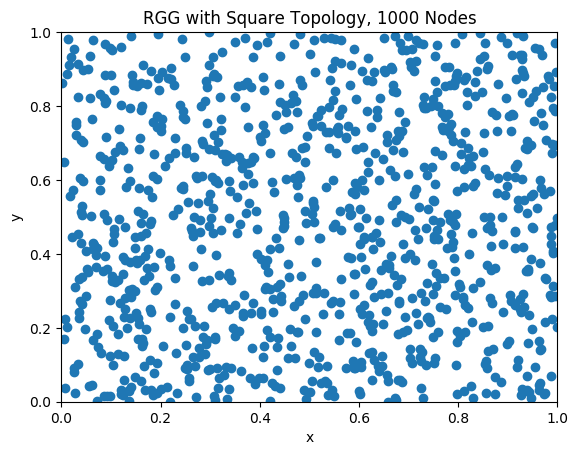
\includegraphics[width=1 \textwidth]{square/drawing/nodes.png}
      \caption{1000 Points on the Square Topology}
    \end{figure}

    \begin{figure}
      \centering
      \label{drawing_of_disc}
      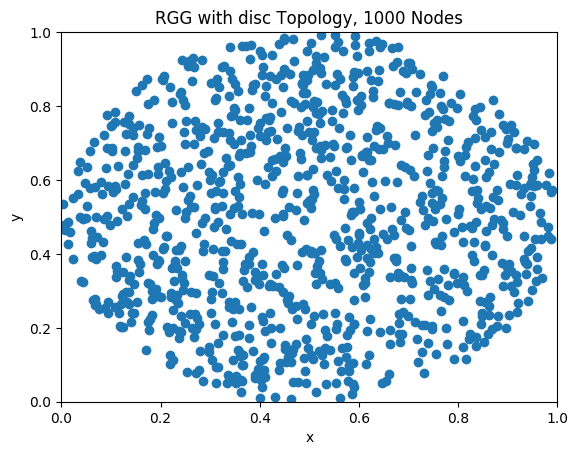
\includegraphics[width=1 \textwidth]{disc/drawing/nodes.png}
      \caption{1000 Points on the Disc Topology}
    \end{figure}
    \begin{figure}
      \centering
      \label{drawing_of_sphere}
      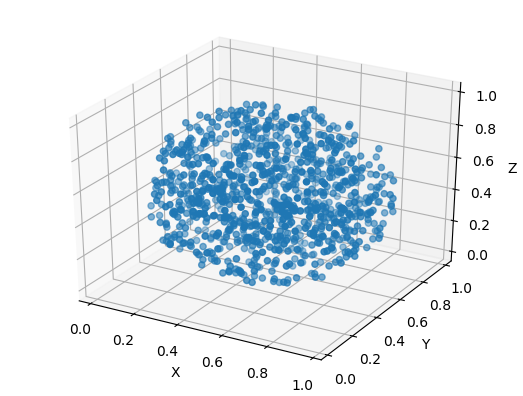
\includegraphics[width=1 \textwidth]{sphere/drawing/sphere_drawing.png}
      \caption{1000 Points on the Sphere Topology}
    \end{figure}

    \paragraph{Edge Density}
    Checking the distribution of the edge densities is one way to verify that the edges are connecting as expected
    The edge distributions should follow a gaussian distribution.
    Figures \ref{square_edge_density}, \ref{disc_edge_density}, and \ref{sphere_edge_density} all show gaussian distrubutions for their respective topologies.
    All of the edge density distributions follow a gaussian distribution which is what is expected meaning that the edges likely connected the nodes in the expected way.

    \begin{figure}
      \centering
      \label{square_edge_density}
      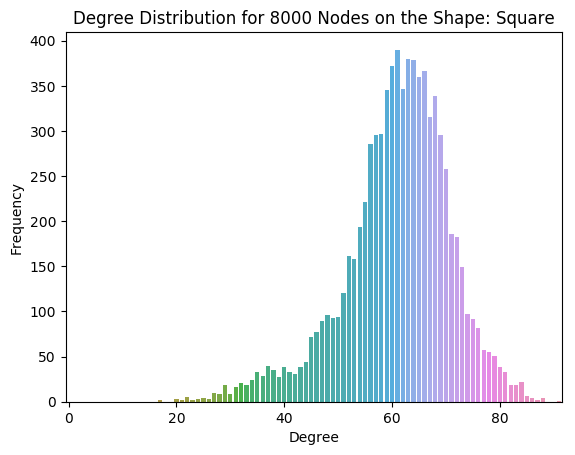
\includegraphics[width=1 \textwidth]{square/edge_density/8000_64.png}
      \caption{Edge Densities of an 8000 Node Graph with E(Degree)=64 on Topology Square}
    \end{figure}

    \begin{figure}
      \centering
      \label{disc_edge_density}
      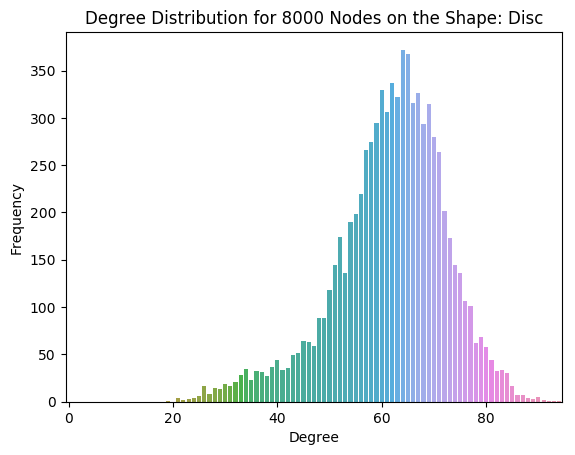
\includegraphics[width=1 \textwidth]{disc/edge_density/8000_64.png}
      \caption{Edge Densities of an 8000 Node Graph with E(Degree)=64 on Topology Disc}
    \end{figure}

    \begin{figure}
      \centering
      \label{sphere_edge_density}
      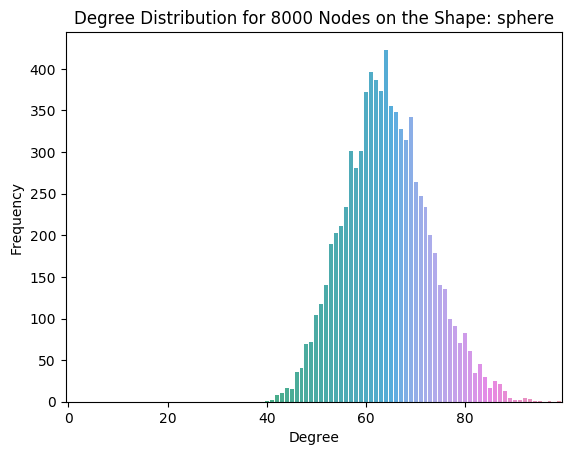
\includegraphics[width=1 \textwidth]{sphere/edge_density/8000_64.png}
      \caption{Edge Densities of an 8000 Node Graph with E(Degree)=64 on Topology Sphere}
    \end{figure}

\section{Result Summary}
  All of my algorithms ran in $O(n)$ time.
  There was variance between the runtime of the different topologies due to the way the points were generated combined with the calculation required to compute 2d distance vs 3d distance.
  Table \ref{runtime_comparison_by_topology} shows the runtime of all of the topologies in a table.
  Figures \ref{square_rgg_runtime_chart}, \ref{disc_rgg_runtime_chart}, and \ref{sphere_rgg_runtime_chart} show the individual runtime charts.
  Figure \ref{all_rgg_runtimes_chart} shows all of the runtimes of the different RGG generation algorithms overlaying each other.
  As discussed in the verification section, multiple plots have been used to verify the accuracy of the algorithms.

  \begin{table}
    \centering
    \label{runtime_comparison_by_topology}
	  \csvautotabular{../results/shared/generation_speeds.csv}
	  \caption{Comparison of Runtimes of Generating the Different Topologies}
  \end{table}

  \begin{figure}
    \centering
    \label{square_rgg_runtime_chart}
    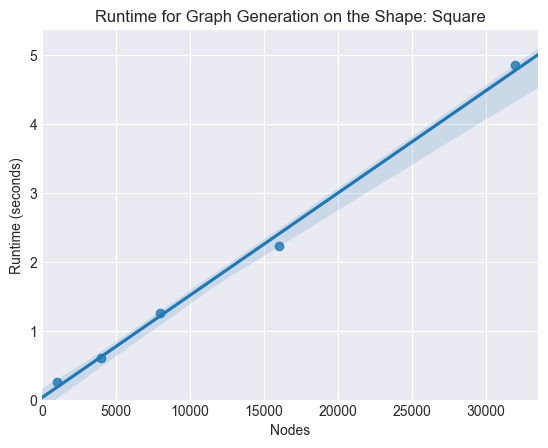
\includegraphics[width=1 \textwidth]{square/runtime/runtime_chart}
    \caption{Runtimes of the $O(n)$ Square RGG Generation Algorithm}
  \end{figure}

  \begin{figure}
    \centering
    \label{disc_rgg_runtime_chart}
    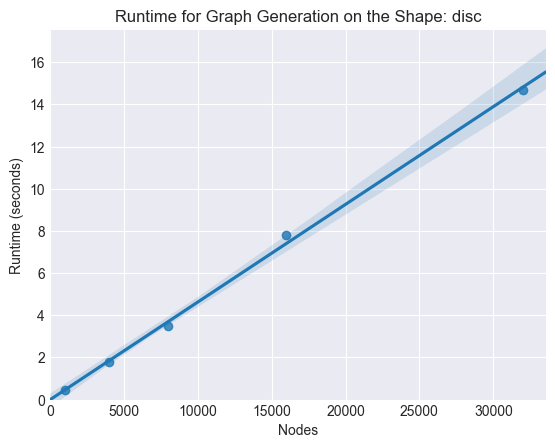
\includegraphics[width=1 \textwidth]{disc/runtime/runtime_chart}
    \caption{Runtimes of the $O(n)$ Disc RGG Generation Algorithm}
  \end{figure}

  \begin{figure}
    \centering
    \label{sphere_rgg_runtime_chart}
    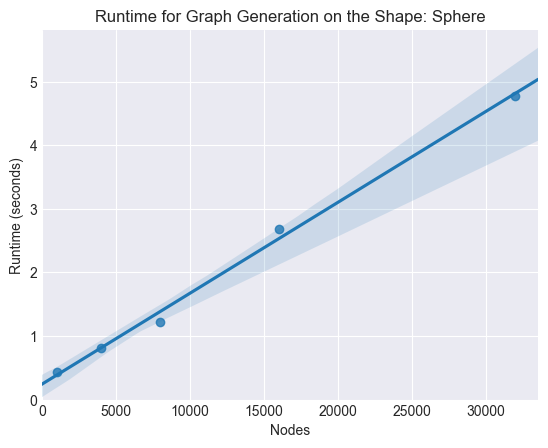
\includegraphics[width=1 \textwidth]{sphere/runtime/runtime_chart}
    \caption{Runtimes of the $O(n)$ Sphere RGG Generation Algorithm}
  \end{figure}

  \begin{figure}
    \centering
    \label{all_rgg_runtimes_chart}
    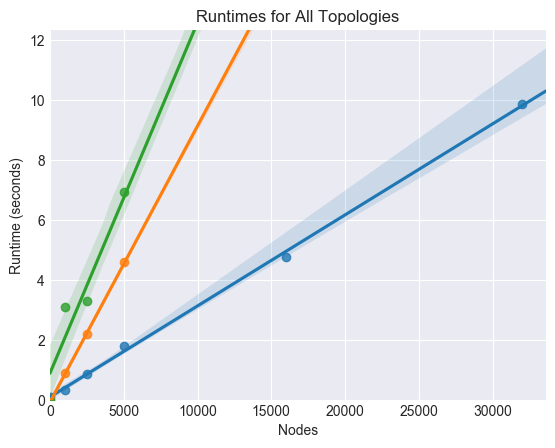
\includegraphics[width=1 \textwidth]{shared/runtime/running_times}
    \caption{Runtimes of the $O(n)$ RGG Generation Algorithms overlayed}
  \end{figure}

\printbibliography

\end{document}
